\documentclass{article}
\usepackage[legalpaper, portrait, margin=0.5in]{geometry}
\usepackage {amsmath}
\usepackage {amssymb}
\usepackage {enumerate}
\usepackage{tikz}
\usetikzlibrary{arrows.meta, positioning, calc}

\title{CSC226 Exercise 11}
\author{Dryden Bryson}
\date{\today}

\begin{document}
\maketitle
\newpage
\section*{Transshipment Problem Graph}
\begin{center}
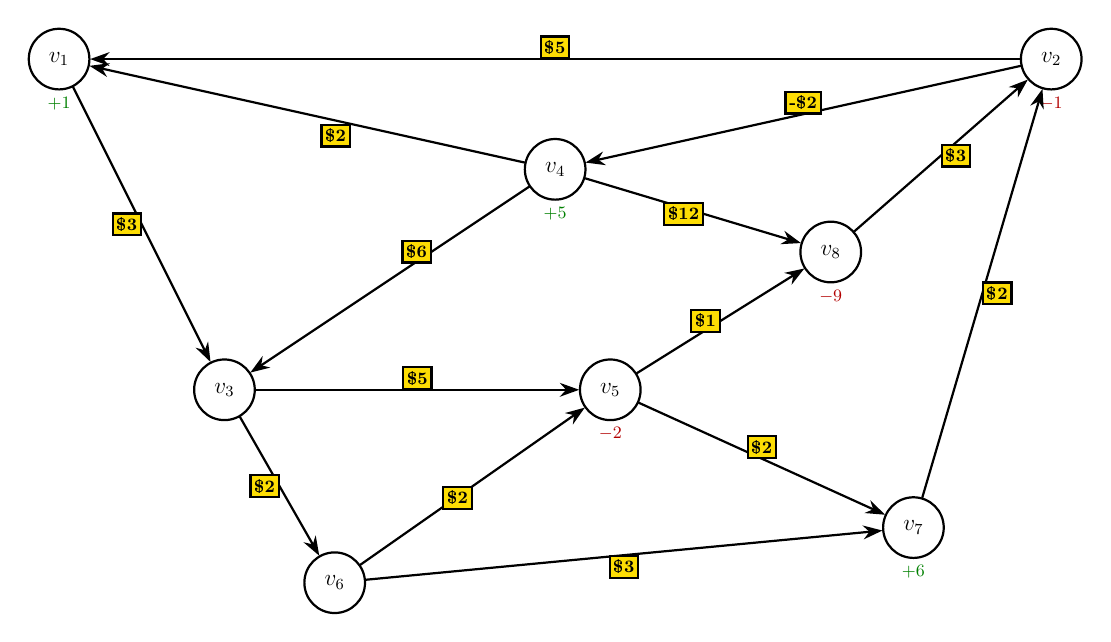
\begin{tikzpicture}[
    scale=0.7,
    transform shape,
    node distance=3cm,
    vertex/.style={
        circle, draw, thick, minimum size=1.1cm, inner sep=0pt,
        font=\large
    },
    cost/.style={
        fill=yellow!80!orange, draw=black, font=\small\bfseries,
        inner sep=2pt, rectangle
    },
    supply/.style={font=\small\bfseries, text=green!50!black},
    demand/.style={font=\small\bfseries, text=red!70!black},
    edge/.style={-{Stealth[length=7pt,width=5pt]}, thick},
]

% Nodes
\node[vertex] (v1) at (0, 8)  {$v_1$};
\node[supply, below=0pt of v1.south, anchor=north] {$+1$};

\node[vertex] (v2) at (18, 8) {$v_2$};
\node[demand, below=0pt of v2.south, anchor=north] {$-1$};

\node[vertex] (v4) at (9, 6) {$v_4$};
\node[supply, below=0pt of v4.south, anchor=north] {$+5$};

\node[vertex] (v3) at (3, 2) {$v_3$};

\node[vertex] (v5) at (10, 2) {$v_5$};
\node[demand, below=0pt of v5.south, anchor=north] {$-2$};

\node[vertex] (v8) at (14, 4.5) {$v_8$};
\node[demand, below=0pt of v8.south, anchor=north] {$-9$};

\node[vertex] (v6) at (5, -1.5) {$v_6$};

\node[vertex] (v7) at (15.5, -0.5) {$v_7$};
\node[supply, below=0pt of v7.south, anchor=north] {$+6$};

% Edges with cost labels

% v2 -> v1 : $5
\draw[edge] (v2) -- node[cost, above, pos=0.5] {\$5} (v1);

% v4 -> v1 : $2
\draw[edge] (v4) -- node[cost, below left, pos=0.4] {\$2} (v1);

% v2 -> v4 : -$2
\draw[edge] (v2) -- node[cost, above, pos=0.5] {-\$2} (v4);

% v8 -> v2 : $3
\draw[edge] (v8) -- node[cost, right, pos=0.5] {\$3} (v2);

% v4 -> v8 : $12
\draw[edge] (v4) -- node[cost, left, pos=0.55] {\$12} (v8);

% v4 -> v3 : $6
\draw[edge] (v4) -- node[cost, left, pos=0.35] {\$6} (v3);

% v1 -> v3 : $3
\draw[edge] (v1) -- node[cost, left, pos=0.5] {\$3} (v3);

% v3 -> v5 : $5
\draw[edge] (v3) -- node[cost, above, pos=0.5] {\$5} (v5);

% v3 -> v6 : $2
\draw[edge] (v3) -- node[cost, left, pos=0.5] {\$2} (v6);

% v6 -> v5 : $2
\draw[edge] (v6) -- node[cost, below left, pos=0.5] {\$2} (v5);

% v5 -> v8 : $1
\draw[edge] (v5) -- node[cost, left, pos=0.5] {\$1} (v8);

% v5 -> v7 : $2
\draw[edge] (v5) -- node[cost, above, pos=0.5] {\$2} (v7);

% v6 -> v7 : $3
\draw[edge] (v6) -- node[cost, below, pos=0.5] {\$3} (v7);

% v7 -> v2 : $2
\draw[edge] (v7) -- node[cost, right, pos=0.5] {\$2} (v2);

\end{tikzpicture}
\end{center}

\section*{Transhipment Solution Graph}
\begin{center}
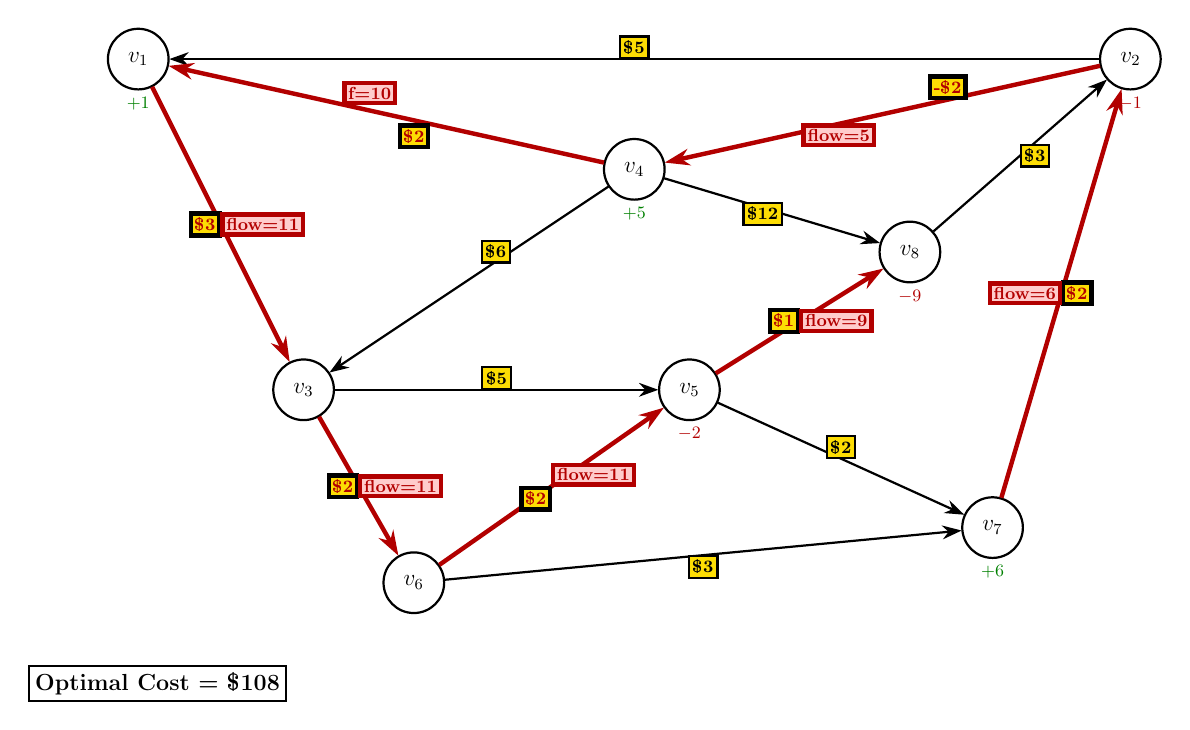
\begin{tikzpicture}[
    scale=0.7,
    transform shape,
    node distance=3cm,
    vertex/.style={
        circle, draw, thick, minimum size=1.1cm, inner sep=0pt,
        font=\large
    },
    cost/.style={
        fill=yellow!80!orange, draw=black, font=\small\bfseries,
        inner sep=2pt, rectangle
    },
    flow/.style={
        fill=red!20, draw=red!70!black, font=\small\bfseries,
        inner sep=2pt, rectangle
    },
    supply/.style={font=\small\bfseries, text=green!50!black},
    demand/.style={font=\small\bfseries, text=red!70!black},
    edge/.style={-{Stealth[length=7pt,width=5pt]}, thick},
    soledge/.style={-{Stealth[length=9pt,width=6pt]}, ultra thick, red!70!black},
]

% Nodes
\node[vertex] (v1) at (0, 8)  {$v_1$};
\node[supply, below=0pt of v1.south, anchor=north] {$+1$};

\node[vertex] (v2) at (18, 8) {$v_2$};
\node[demand, below=0pt of v2.south, anchor=north] {$-1$};

\node[vertex] (v4) at (9, 6) {$v_4$};
\node[supply, below=0pt of v4.south, anchor=north] {$+5$};

\node[vertex] (v3) at (3, 2) {$v_3$};

\node[vertex] (v5) at (10, 2) {$v_5$};
\node[demand, below=0pt of v5.south, anchor=north] {$-2$};

\node[vertex] (v8) at (14, 4.5) {$v_8$};
\node[demand, below=0pt of v8.south, anchor=north] {$-9$};

\node[vertex] (v6) at (5, -1.5) {$v_6$};

\node[vertex] (v7) at (15.5, -0.5) {$v_7$};
\node[supply, below=0pt of v7.south, anchor=north] {$+6$};

% Non-solution edges (normal style)

% v2 -> v1 : $5
\draw[edge] (v2) -- node[cost, above, pos=0.5] {\$5} (v1);

% v8 -> v2 : $3
\draw[edge] (v8) -- node[cost, right, pos=0.5] {\$3} (v2);

% v4 -> v8 : $12
\draw[edge] (v4) -- node[cost, left, pos=0.55] {\$12} (v8);

% v4 -> v3 : $6
\draw[edge] (v4) -- node[cost, left, pos=0.35] {\$6} (v3);

% v3 -> v5 : $5
\draw[edge] (v3) -- node[cost, above, pos=0.5] {\$5} (v5);

% v5 -> v7 : $2
\draw[edge] (v5) -- node[cost, above, pos=0.5] {\$2} (v7);

% v6 -> v7 : $3
\draw[edge] (v6) -- node[cost, below, pos=0.5] {\$3} (v7);

% Solution edges (red, ultra thick, with flow labels)

% v4 -> v1 : $2, flow=10
\draw[soledge] (v4) -- node[cost, below left, pos=0.4] {\$2} node[flow, above right, pos=0.6] {f=10} (v1);

% v2 -> v4 : -$2, flow=5
\draw[soledge] (v2) -- node[cost, above, pos=0.35] {-\$2} node[flow, below, pos=0.6] {flow=5} (v4);

% v1 -> v3 : $3, flow=11
\draw[soledge] (v1) -- node[cost, left, pos=0.5] {\$3} node[flow, right, pos=0.5] {flow=11} (v3);

% v3 -> v6 : $2, flow=11
\draw[soledge] (v3) -- node[cost, left, pos=0.5] {\$2} node[flow, right, pos=0.5] {flow=11} (v6);

% v6 -> v5 : $2, flow=11
\draw[soledge] (v6) -- node[cost, below left, pos=0.5] {\$2} node[flow, above right, pos=0.5] {flow=11} (v5);

% v5 -> v8 : $1, flow=9
\draw[soledge] (v5) -- node[cost, left, pos=0.5] {\$1} node[flow, right, pos=0.5] {flow=9} (v8);

% v7 -> v2 : $2, flow=6
\draw[soledge] (v7) -- node[cost, right, pos=0.5] {\$2} node[flow, left, pos=0.5] {flow=6} (v2);

% Total cost annotation
\node[draw, fill=white, thick, font=\large\bfseries, anchor=north west] at (-2, -3) {Optimal Cost = \$108};

\end{tikzpicture}
\end{center}
\end{document}